\chapter{Results}
\section{Asymmetries in $\theta_{abs}$ of Neutron Singles}
Using data acquired during this study, it is possible to construct $\theta_{abs}$ distributions of neutron singles, where $\theta_{abs}$ is defined as the angle between a neutron's reconstructed direction of travel and the direction of the incident photon beam.
Because the experimental design was motivated by measurements of correlated neutron doubles, not neutron singles, the methods required to obtain a neutron singles measurement are far less robust than for neutron doubles.
Nonetheless, neutron singles measurements from the photo-disintegration of D$_{2}$O showed fair agreement with known values, so the results are not totally without merit.

These distributions were calculated by normalizing the yields of photo-neutrons to the yield of neutrons from SF of $^{252}$Cf, which have no preferred direction.
However, these two yields were measured under very different experimental conditions.
This is different from the case of two-neutron opening angle measurements, which uses the same set of neutron events to generate two yields--uncorrected yield and correlated yield.
Another difference is that the uncorrected yield can be used to subtract accidentals, which includes noise.

 Due to differences in experimental conditions that existed during measurements of photo-neutrons and measurements of neutrons from the SF of $^{252}$Cf, there is a high potential for systematic errors.
The photo-neutron data must be corrected for detector dead-time, which, due to the presence of the photon beam, was about an order of magnitude higher for photo-neutron measurements than for $^{252}$Cf measurements.
Accidental coincidences caused by noise and photons was estimated from data taken with a non-neutron producing aluminum target, which had to be corrected for dead-time and scaled to account for the fact that the aluminum and photo-neutron data sets have different gamma detection rates, and then the result was subtracted from the photo-neutron data.
Furthermore, neutrons from the SF of $^{252}$Cf do not have the same energy distribution as photo-neutrons, which could lead to incorrect results.

Despite all this, the $\theta_{abs}$ distribution for D$_{2}$O agrees fairly well with the previously established distribution, but note that the same may not necessarily be true for $^{238}$U and $^{232}$Th, which have a signal-to-noise ratio that is about 7 and 100 times less than for D$_{2}$O, respectively.

\begin{figure}
    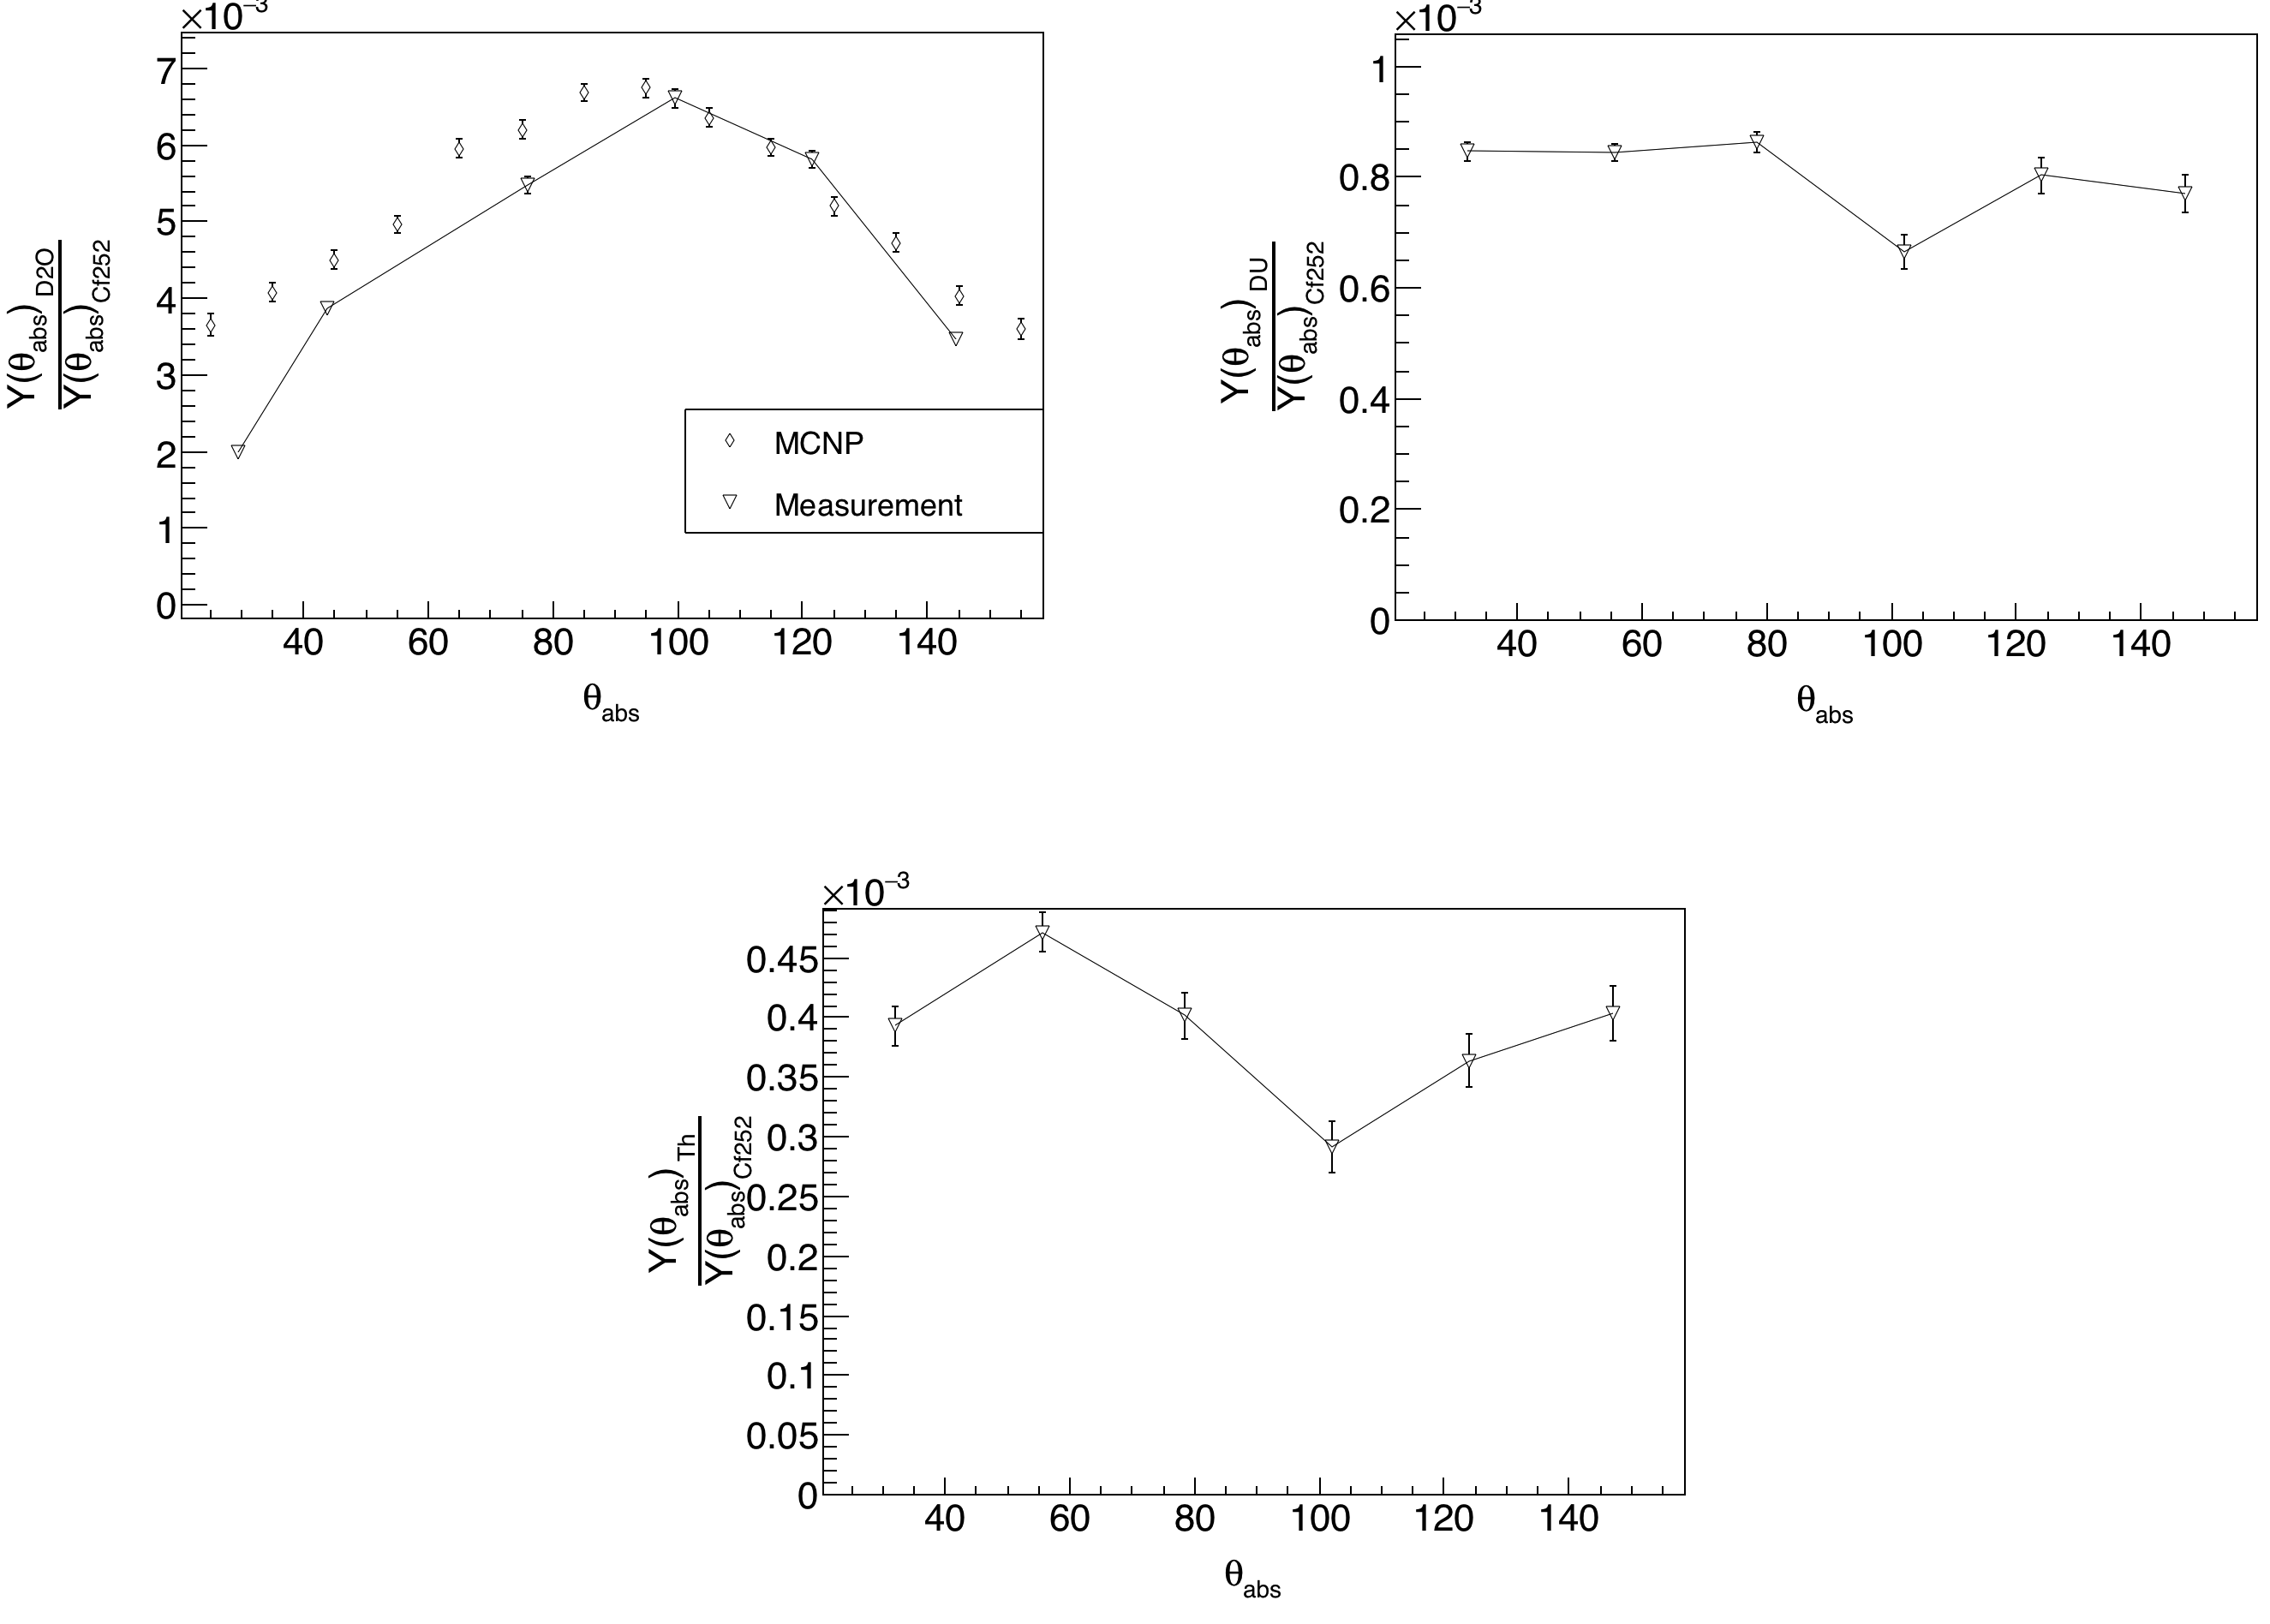
\includegraphics[width = 1\textwidth]{Content/Results/Singles.png}
    \caption{Accessory calculations were performed of the relative rates of neutrons singles as a function of $\theta_{abs}$. 
    Results are expressed as a ratio of the yield of photo-neutron singles from D$_{2}O$, $^{238}$U (DU), and $^{232}$Th, to the yield of neutron singles from the SF of $^{252}$Cf.
   The result for D$_{2}$O is in fair agreement with past measurements, however, these results have high potential for systematic errors due to the differences in experimental conditions under which the yields in the numerator and denominator were measured.
       }
    \label{fig:Singles}
\end{figure}

\FloatBarrier
\section{Two-neutron opening angle correlations}
Some of the results presented here are compared with output from FREYA (Fission Reaction Event Yield Algorithm). 
FREYA was developed by the collaborative efforts of researchers from Lawrence Berkeley National Laboratory,  Lawrence Livermore National Laboratory, Los Almost National Laboratory, and University of Michigan Nuclear Engineering.
It has been included in MCNP since version 6.2 .
All analysis performed on the measured data also applied to the data output by FREYA, with the exception of accidental subtraction.
This includes the normalization to uncorrelated neutrons and the weighting procedures that are described in section~\ref{Analysis}.
 
The most recent release of FREYA, version 2.0.3, does not model photofission directly, but instead uses a neutron-induced fission model to approximate photofission~\cite{FREYA_photofission}.
For a given nucleus with Z protons and A total nucleons, the code selects the neutron-induced fission model for the Z(A-1) nucleus, and chooses an incident neutron energy such that the compound ZA nucleus will have an excitation energy, relative to the ground state of ZA, that is equal to the energy of the incident photon.
All model parameters, such as level density and partition parameters, were set to their default values for neutron-induced fission.
FREYA was told to use the fission fragment mass distribution $Y(A)$ and the average total kinetic energy $\langle$TKE$\rangle(A)$ from the photofission of $^{238}$U, which was taken from the work discussed in ref~\cite{2017Krishichayan}.

In ref~\cite{Talou2018}, the authors warn that using FREYA in this way to model photofission is only an approximation and could lead to incorrect results.
Nonetheless, the approximation is presented here because it is the only photofission model available to the authors of the present work.

The measured $\theta_{nn}$ distribution from the photofission of $^{238}$U and the SF of $^{252}$Cf are presented with the following three different types of cuts applied to the energies of neutrons in coincidence:
\begin{enumerate}[label=(\roman*), itemjoin={{, }}, itemjoin*={{, or }}]
    \item A minimum energy threshold is applied to both neutrons (Figs.~\ref{fig:DU(2)}($^{238}$U) and~\ref{fig:Cf(2)}($^{252}$Cf))
   \item The mean energy of the two neutrons must fall within a specified range ((Figs.~\ref{fig:DU(1)}($^{238}$U) and~\ref{fig:Cf(1)}($^{252}$Cf))
   \item The energy of both neutrons must fall within a specified range (Figs.~\ref{fig:DU(0)}($^{238}$U) and~\ref{fig:Cf(0)}($^{252}$Cf))
  \end{enumerate}
For each type of energy cut, with the exception of case (i), three (four for $^{252}$Cf) mutually exclusive ranges are chosen such that each contains an equal number of events.

When using a histogram to estimate a continuous distribution from the relatively small number of data points obtained of neutrons from the photofission of $^{238}$U, one faces the following dilemma: small bins produce histograms with large uncertainties that are highly dependent on the chosen bin-width, while large bins obscure potentially useful information. 
For this reason, kernel density estimates (KDE) are plotted alongside histograms.
A KDE is a method for estimating a continuous probability distribution from a finite set of sampled data points.
The kernel was chosen to be the known measurements errors in opening angle as determined by the use of a highly collimated $^{60}$Co source, which are well-described by a gaussian with a sigma that varies with $\theta_{nn}$ according to the data presented in Fig.~\ref{fig:OpeningAngleRes}.
Mathematical details of the KDE method used in this work are outlined in ref~\cite{KDE}. 
Alongside each measurement is the result of a FREYA simulation with the exact same energy cuts applied.

For $^{238}$U, there were a total of 2952 two-neutron coincidences events after the subtraction of accidentals.
For $^{252}$Cf, there were a total of 21,882 two-neutron coincidences.


\FloatBarrier
\begin{figure}
\centering
    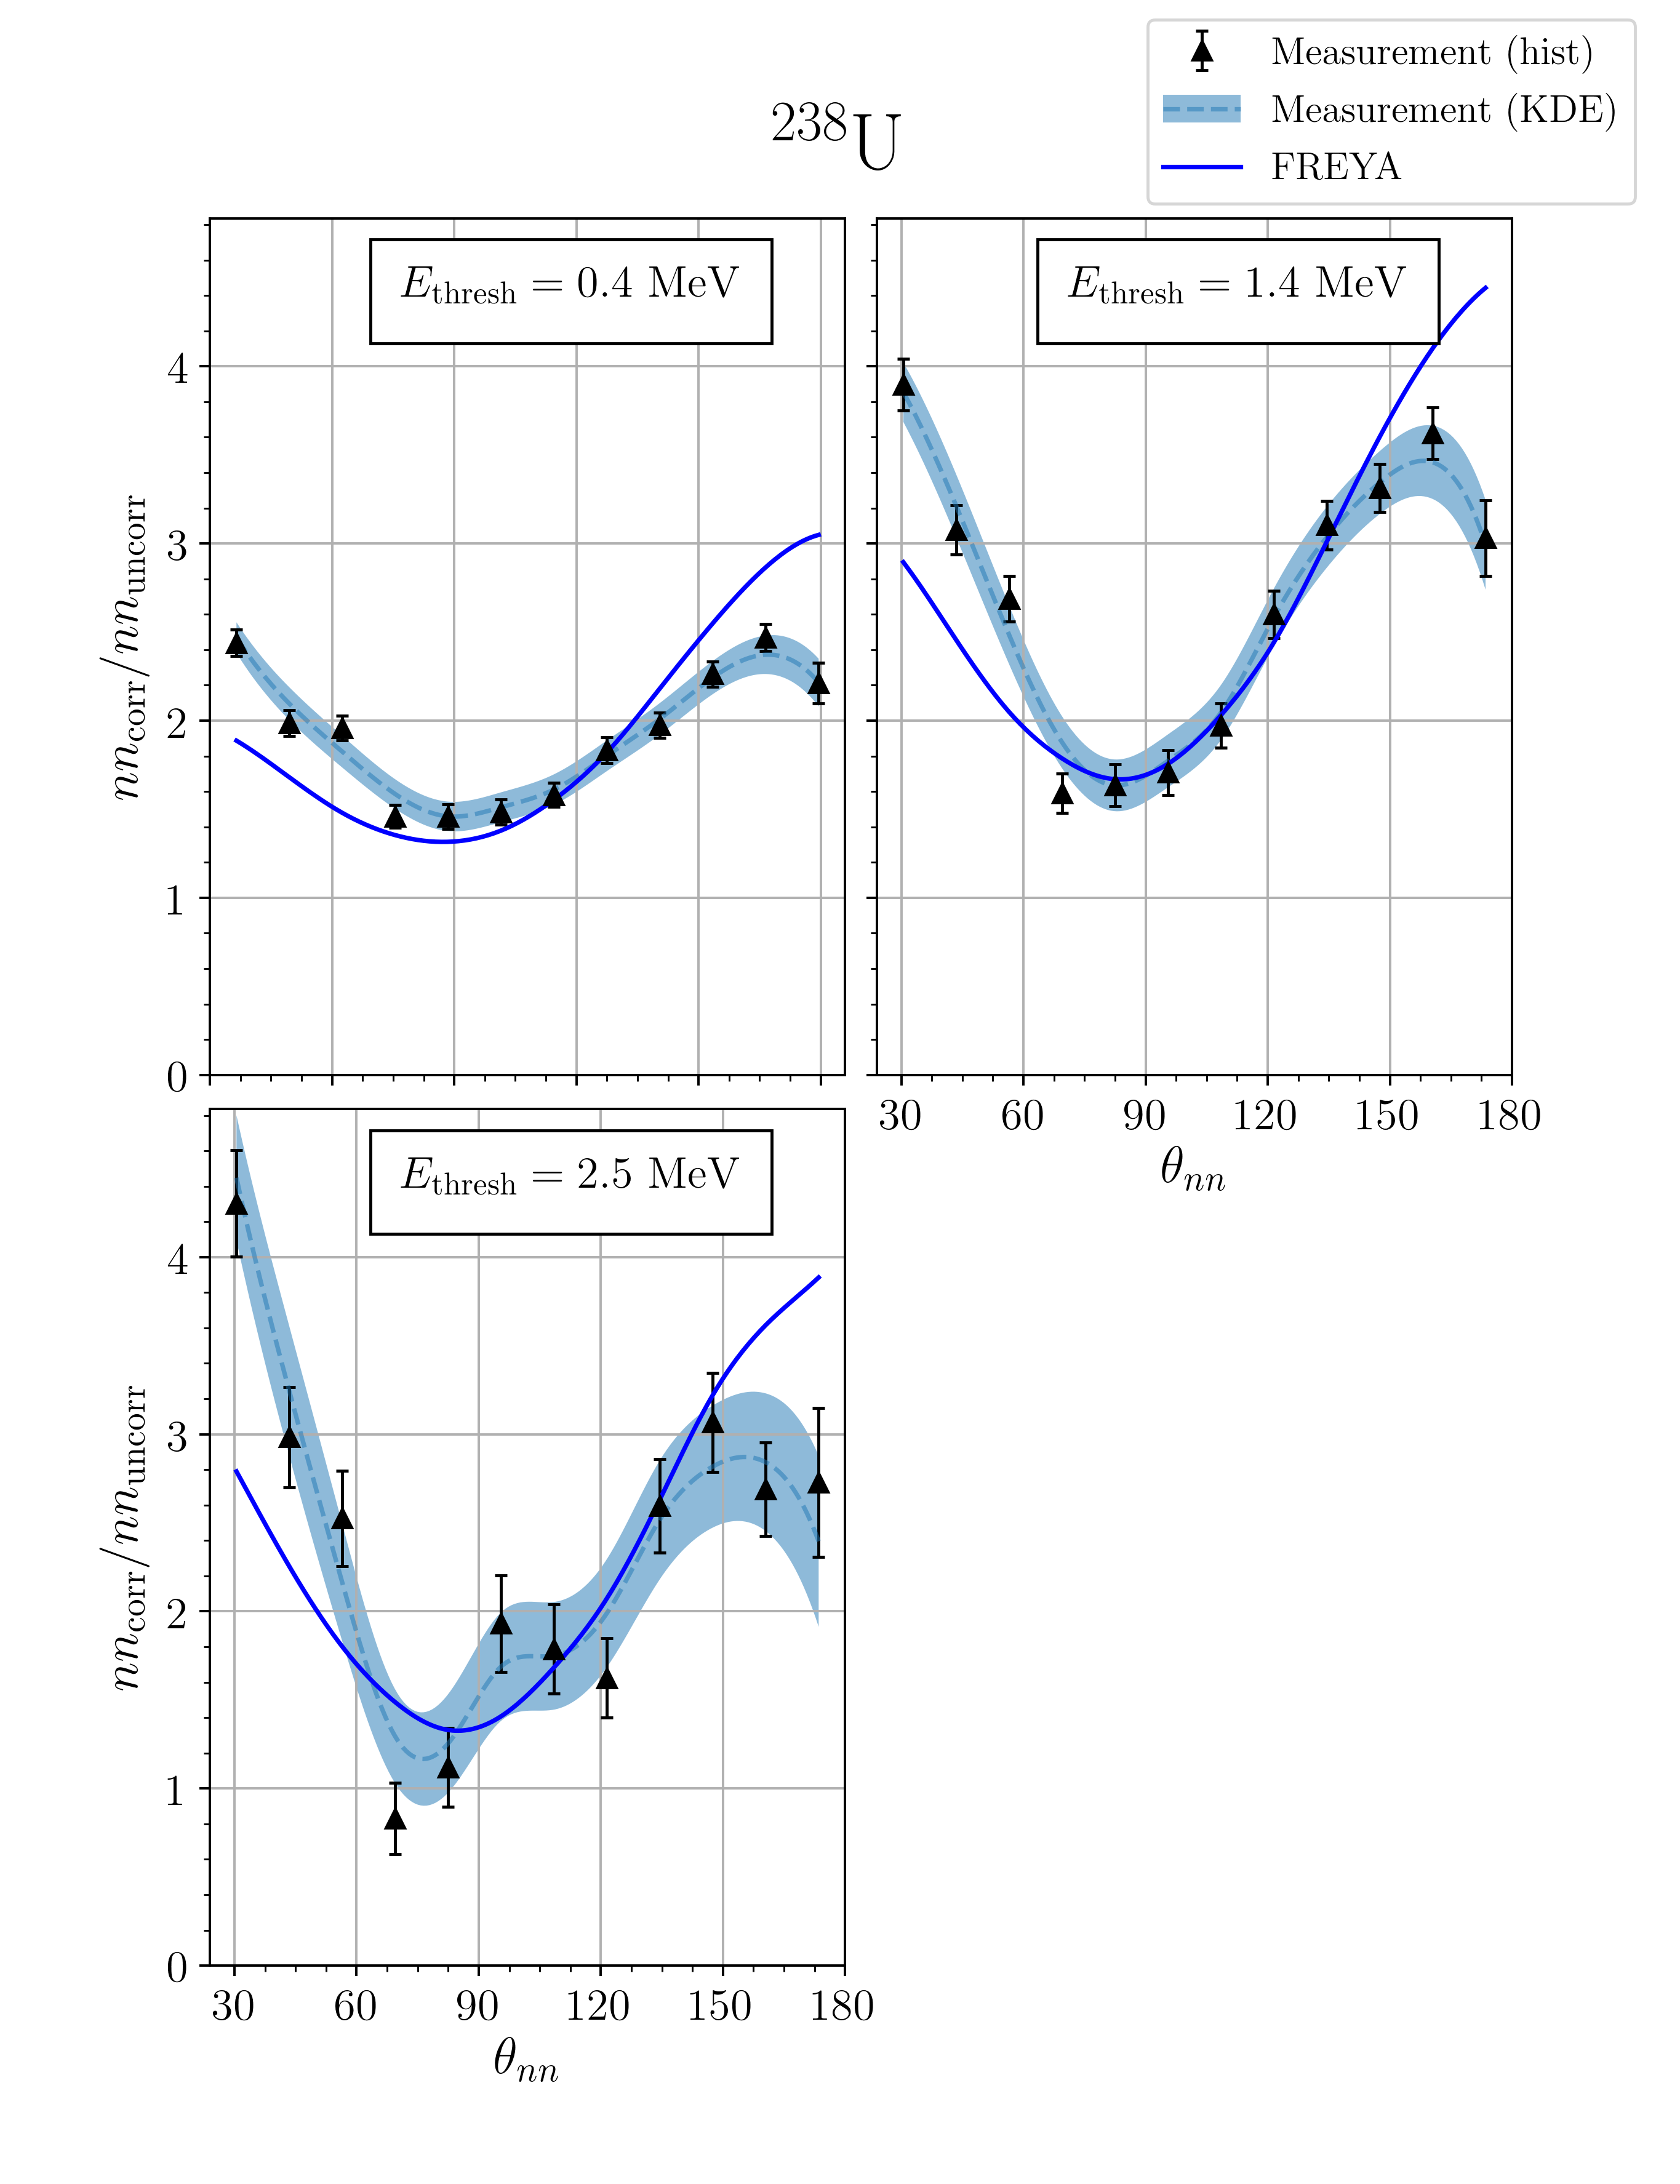
\includegraphics[width = 1.1\textwidth]{Content/Results/FinalDUResultw_freya0KDE.png}
    \caption{$\theta{nn}$ distribution  a minimum energy threshold applied to both neutrons.
    Histogram and kernel density estimate with 68\% confidence interval shown.
    Starting from the lower left and moving counterclockwise, the number of events contributing the each plot are: 314, 2952, 1489 }
    \label{fig:DU(0)}
\end{figure}
\begin{figure}
\centering
    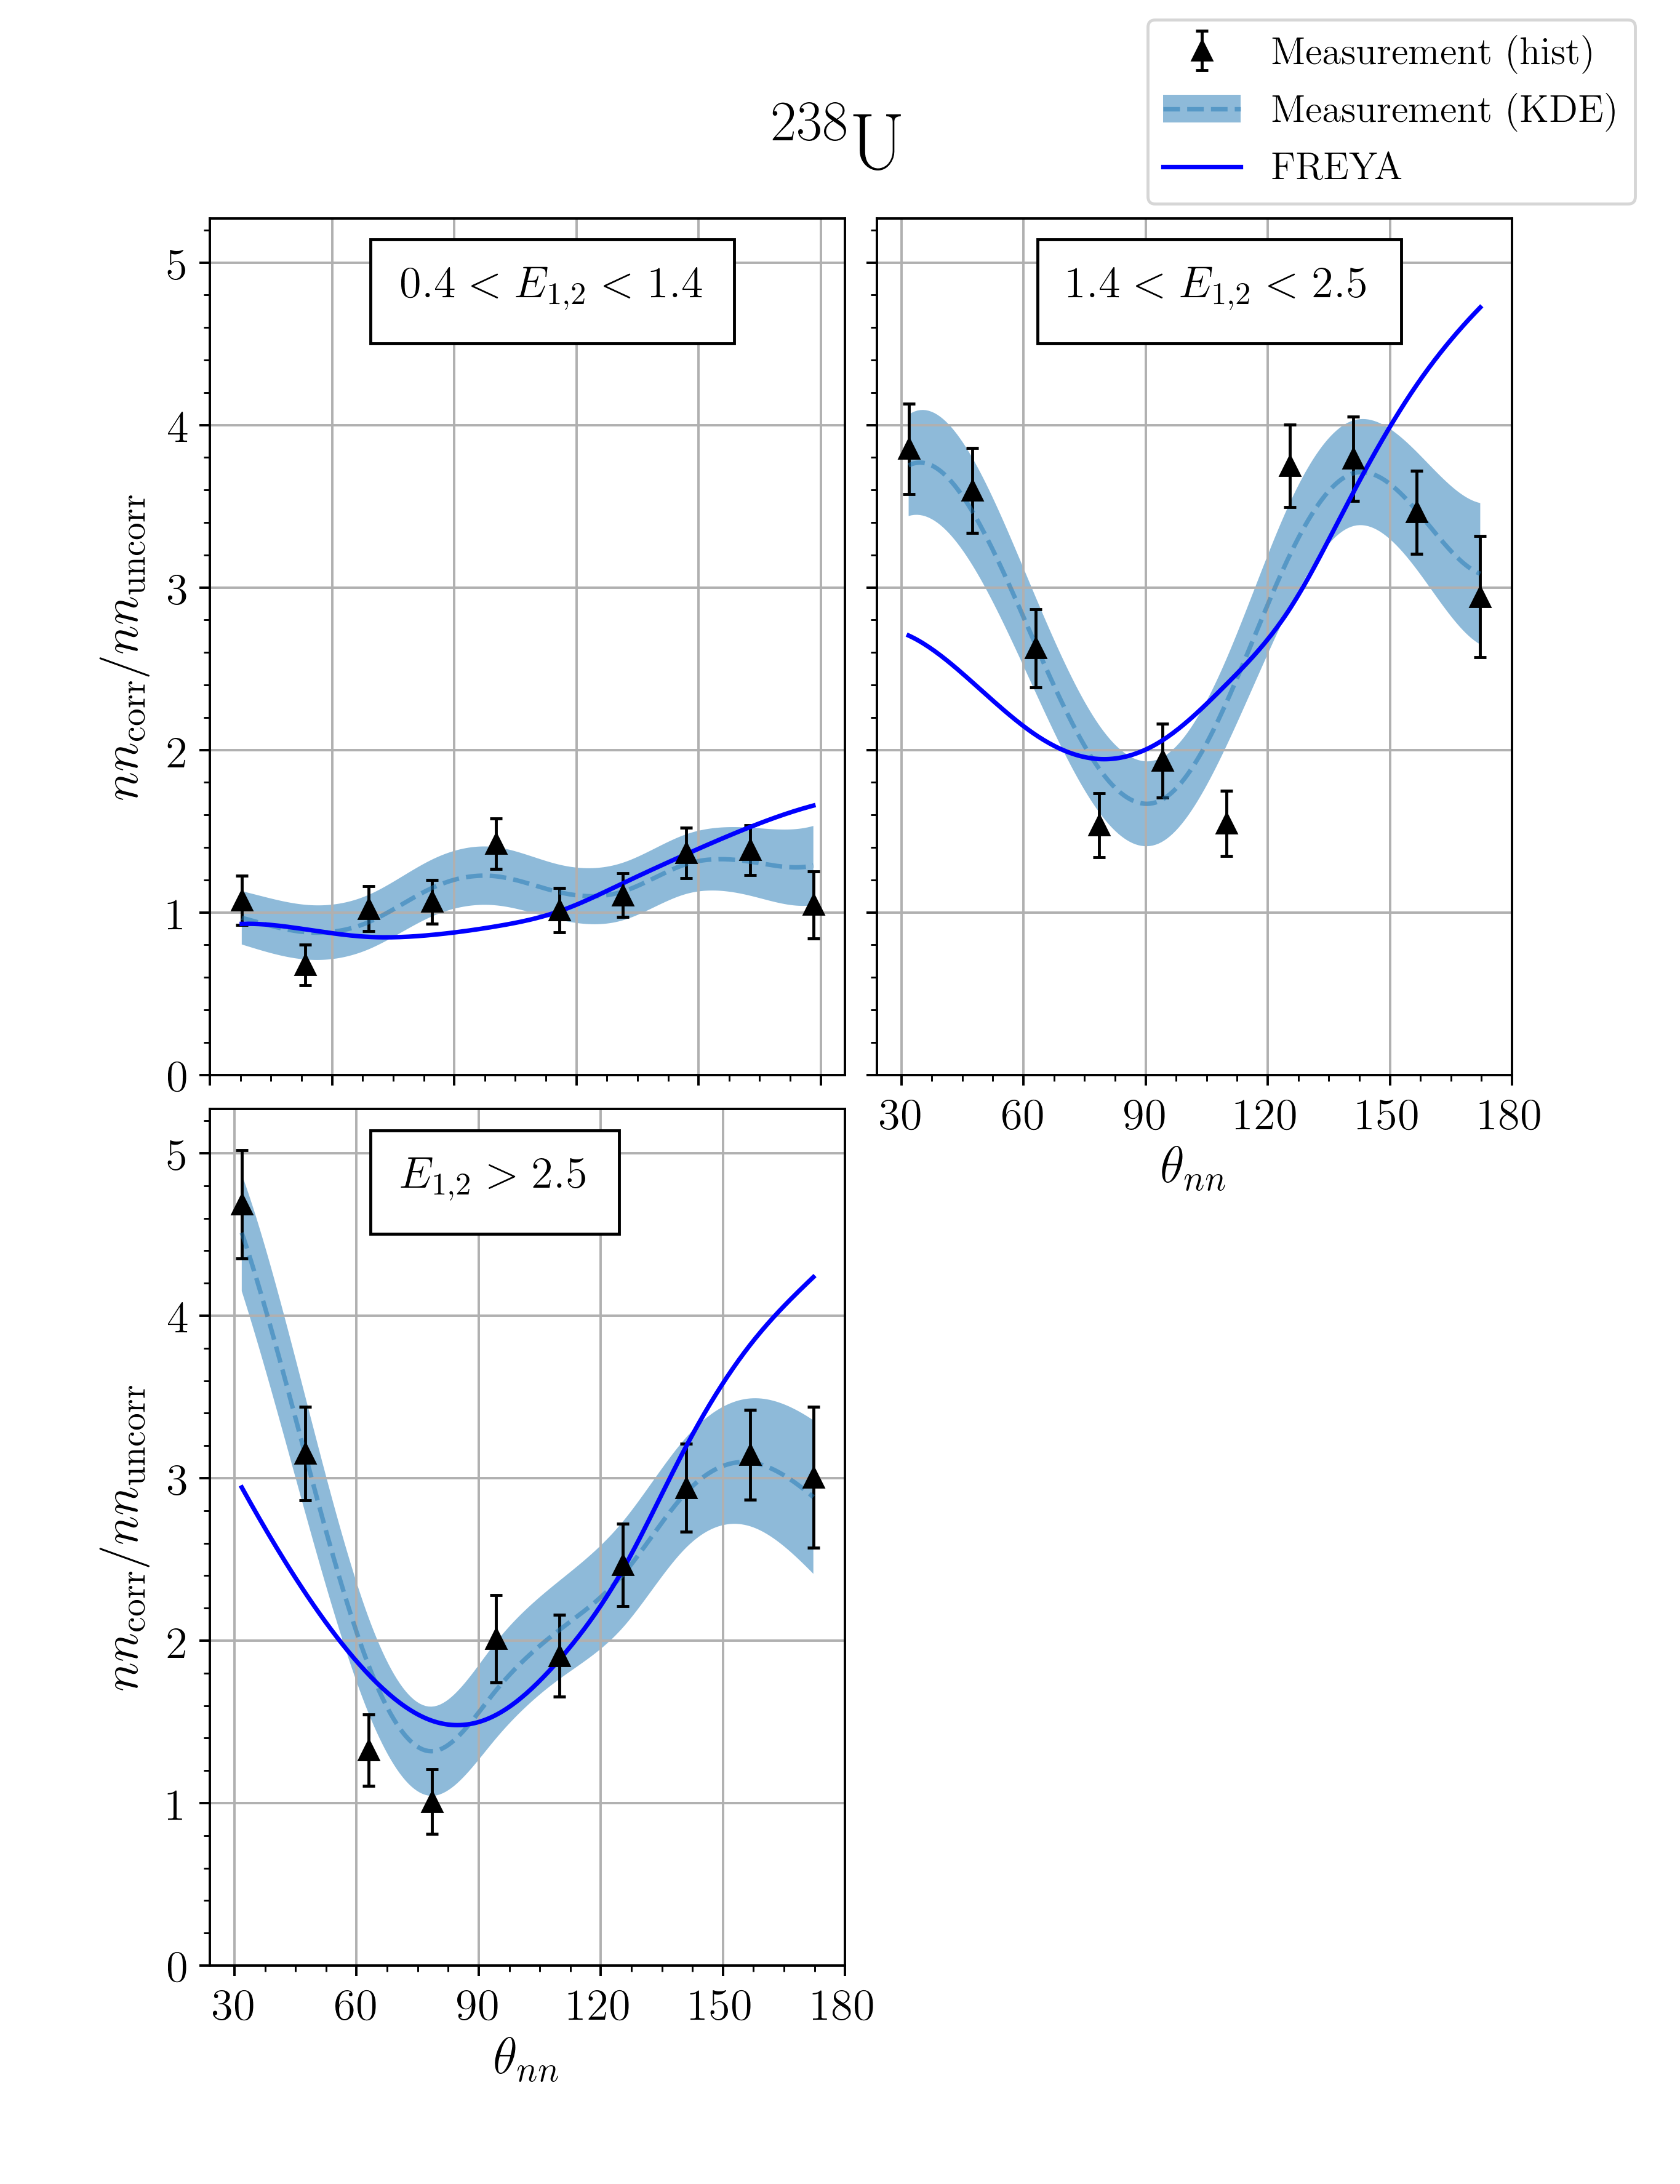
\includegraphics[width = 1.1\textwidth]{Content/Results/FinalDUResultw_freya2KDE.png}
    \caption{ $\theta{nn}$ distribution with cuts on the energies of both coincident neutrons, $E_{1,2}$.
    Histogram and kernel density estimate with 68\% confidence interval shown.
    Starting from the lower left and moving counterclockwise, the number of events contributing the each plot are: 303, 266, and 433.}
    \label{fig:DU(2)}
\end{figure}
\begin{figure}
\centering
    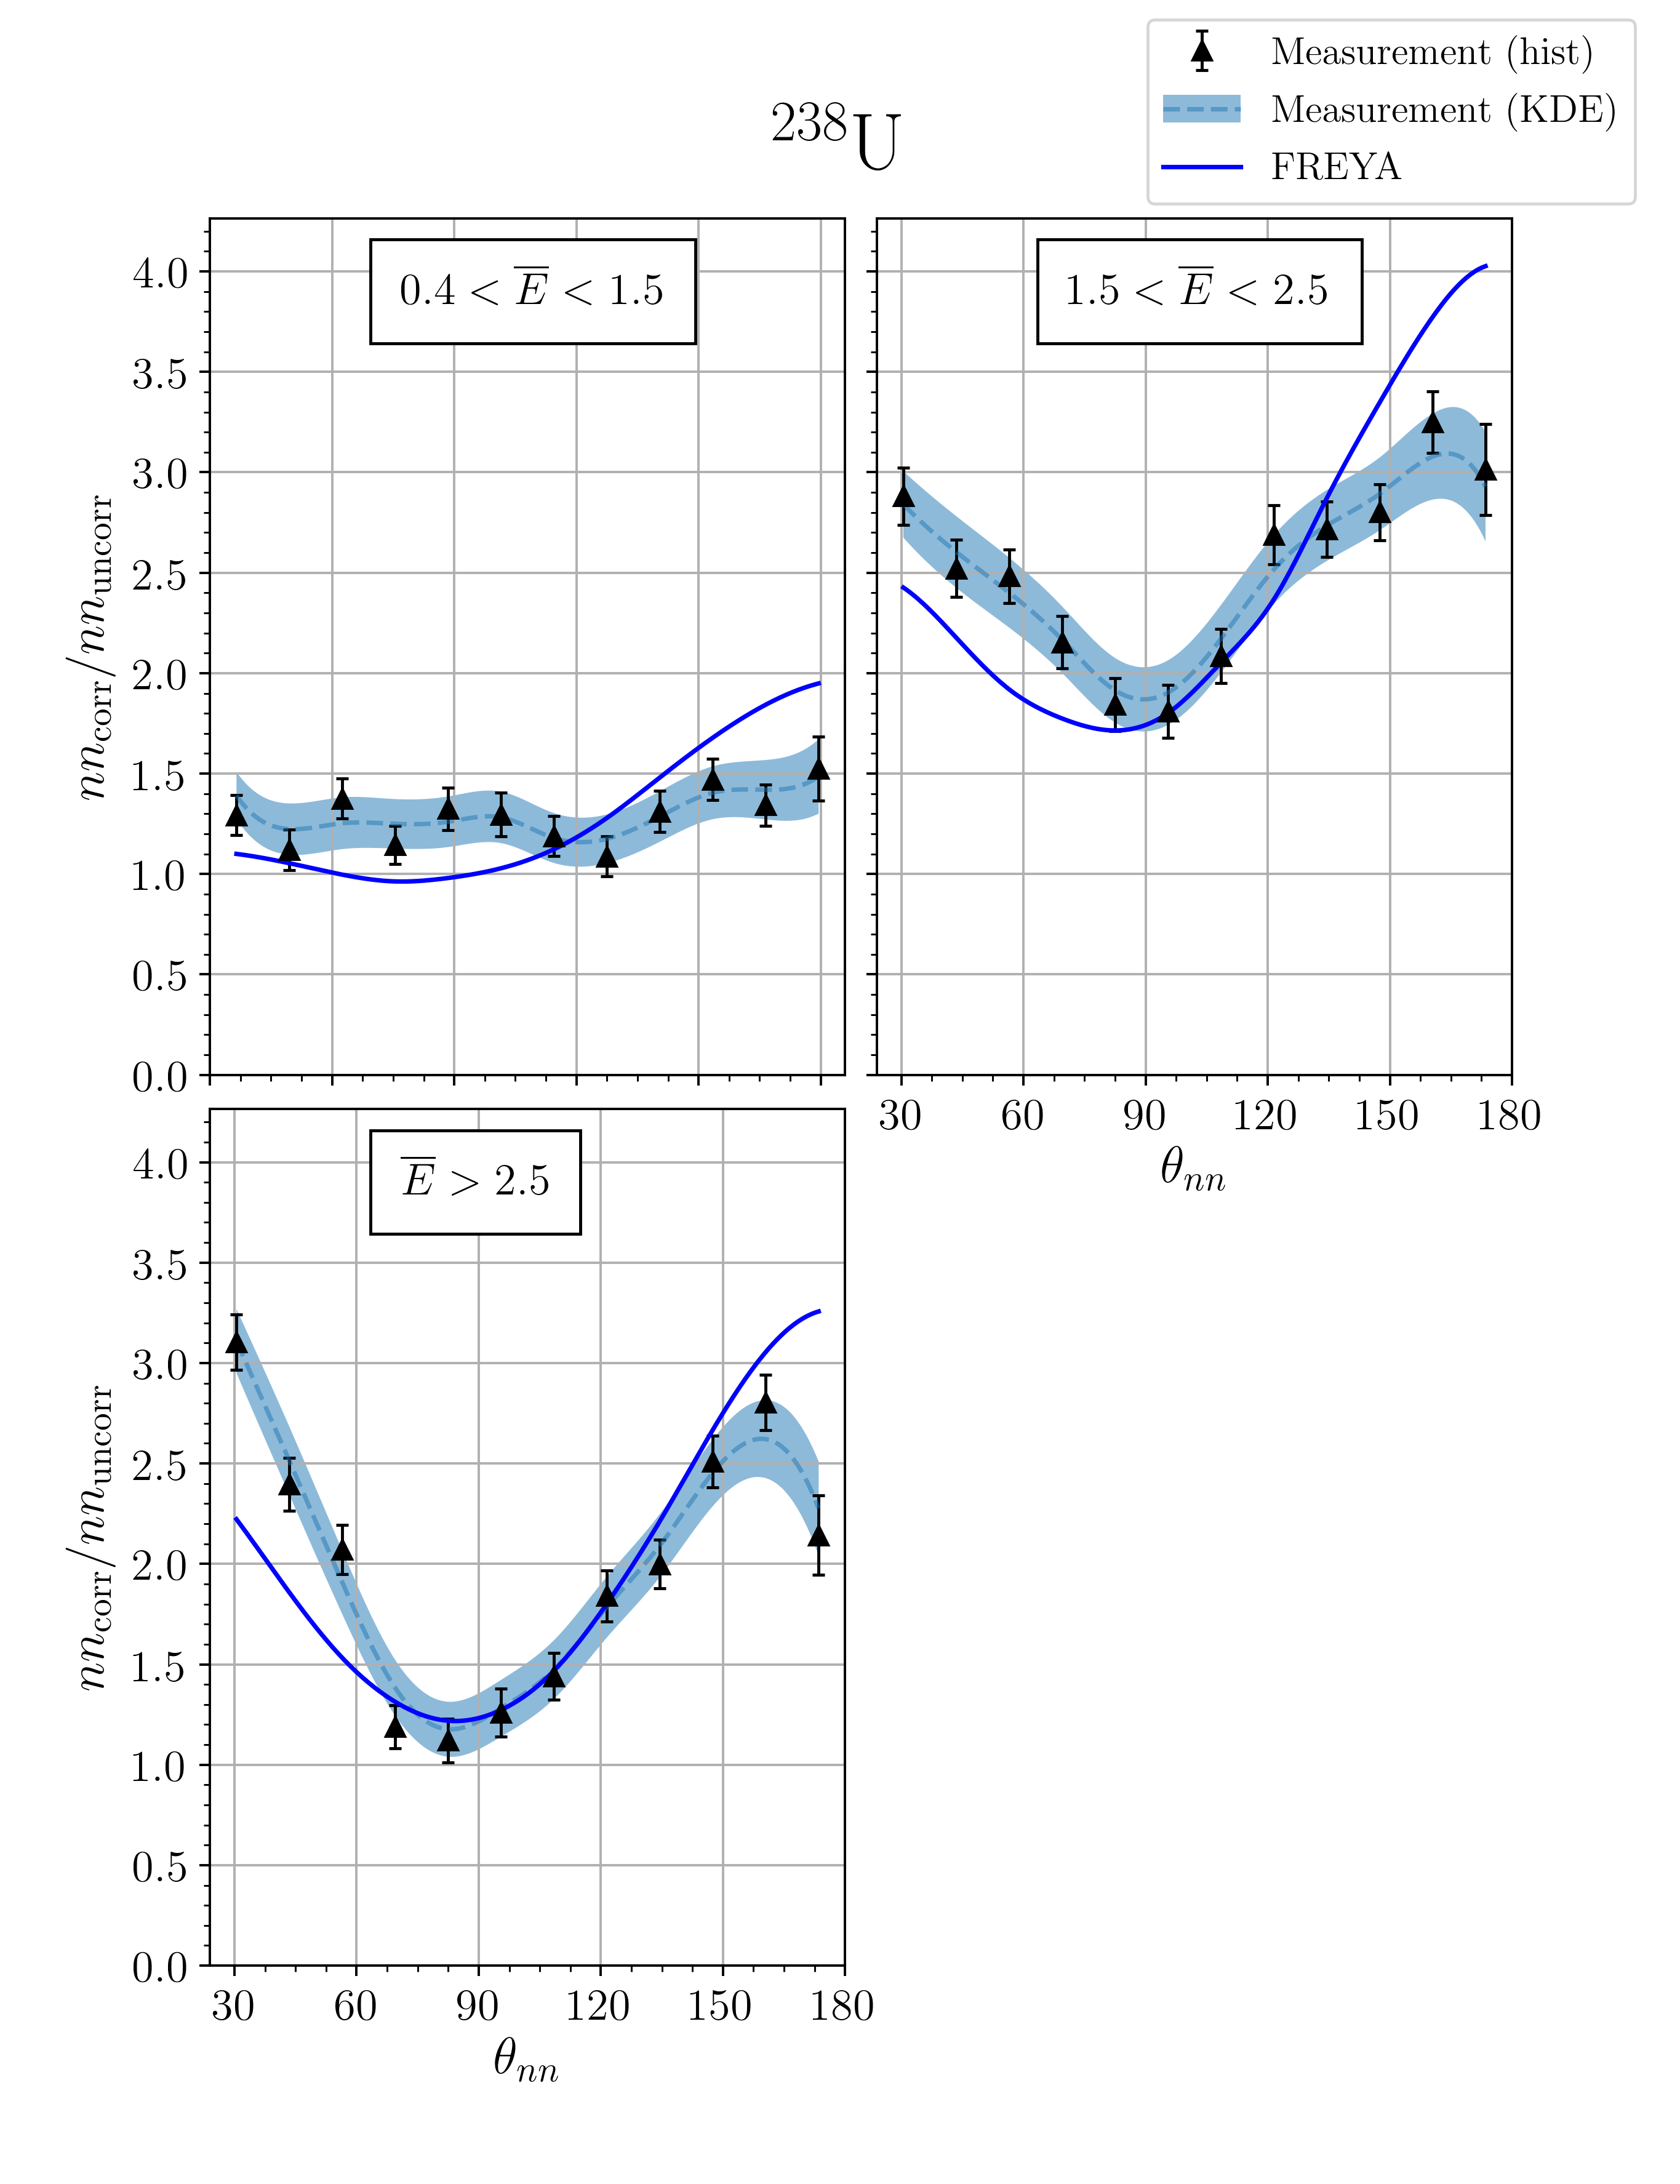
\includegraphics[width = 1.1\textwidth]{Content/Results/FinalDUResultw_freya1KDE.png}
    \caption{$\theta{nn}$ distribution with cuts on the mean energy ($\overline{E}$) of the two coincident neutrons.
    Histogram and kernel density estimate with 68\% confidence interval shown.
    Starting from the lower left and moving counterclockwise, the number of events contributing the each plot are: 1009, 756, 1187 }
    \label{fig:DU(1)}
\end{figure}

\begin{figure}
\centering
    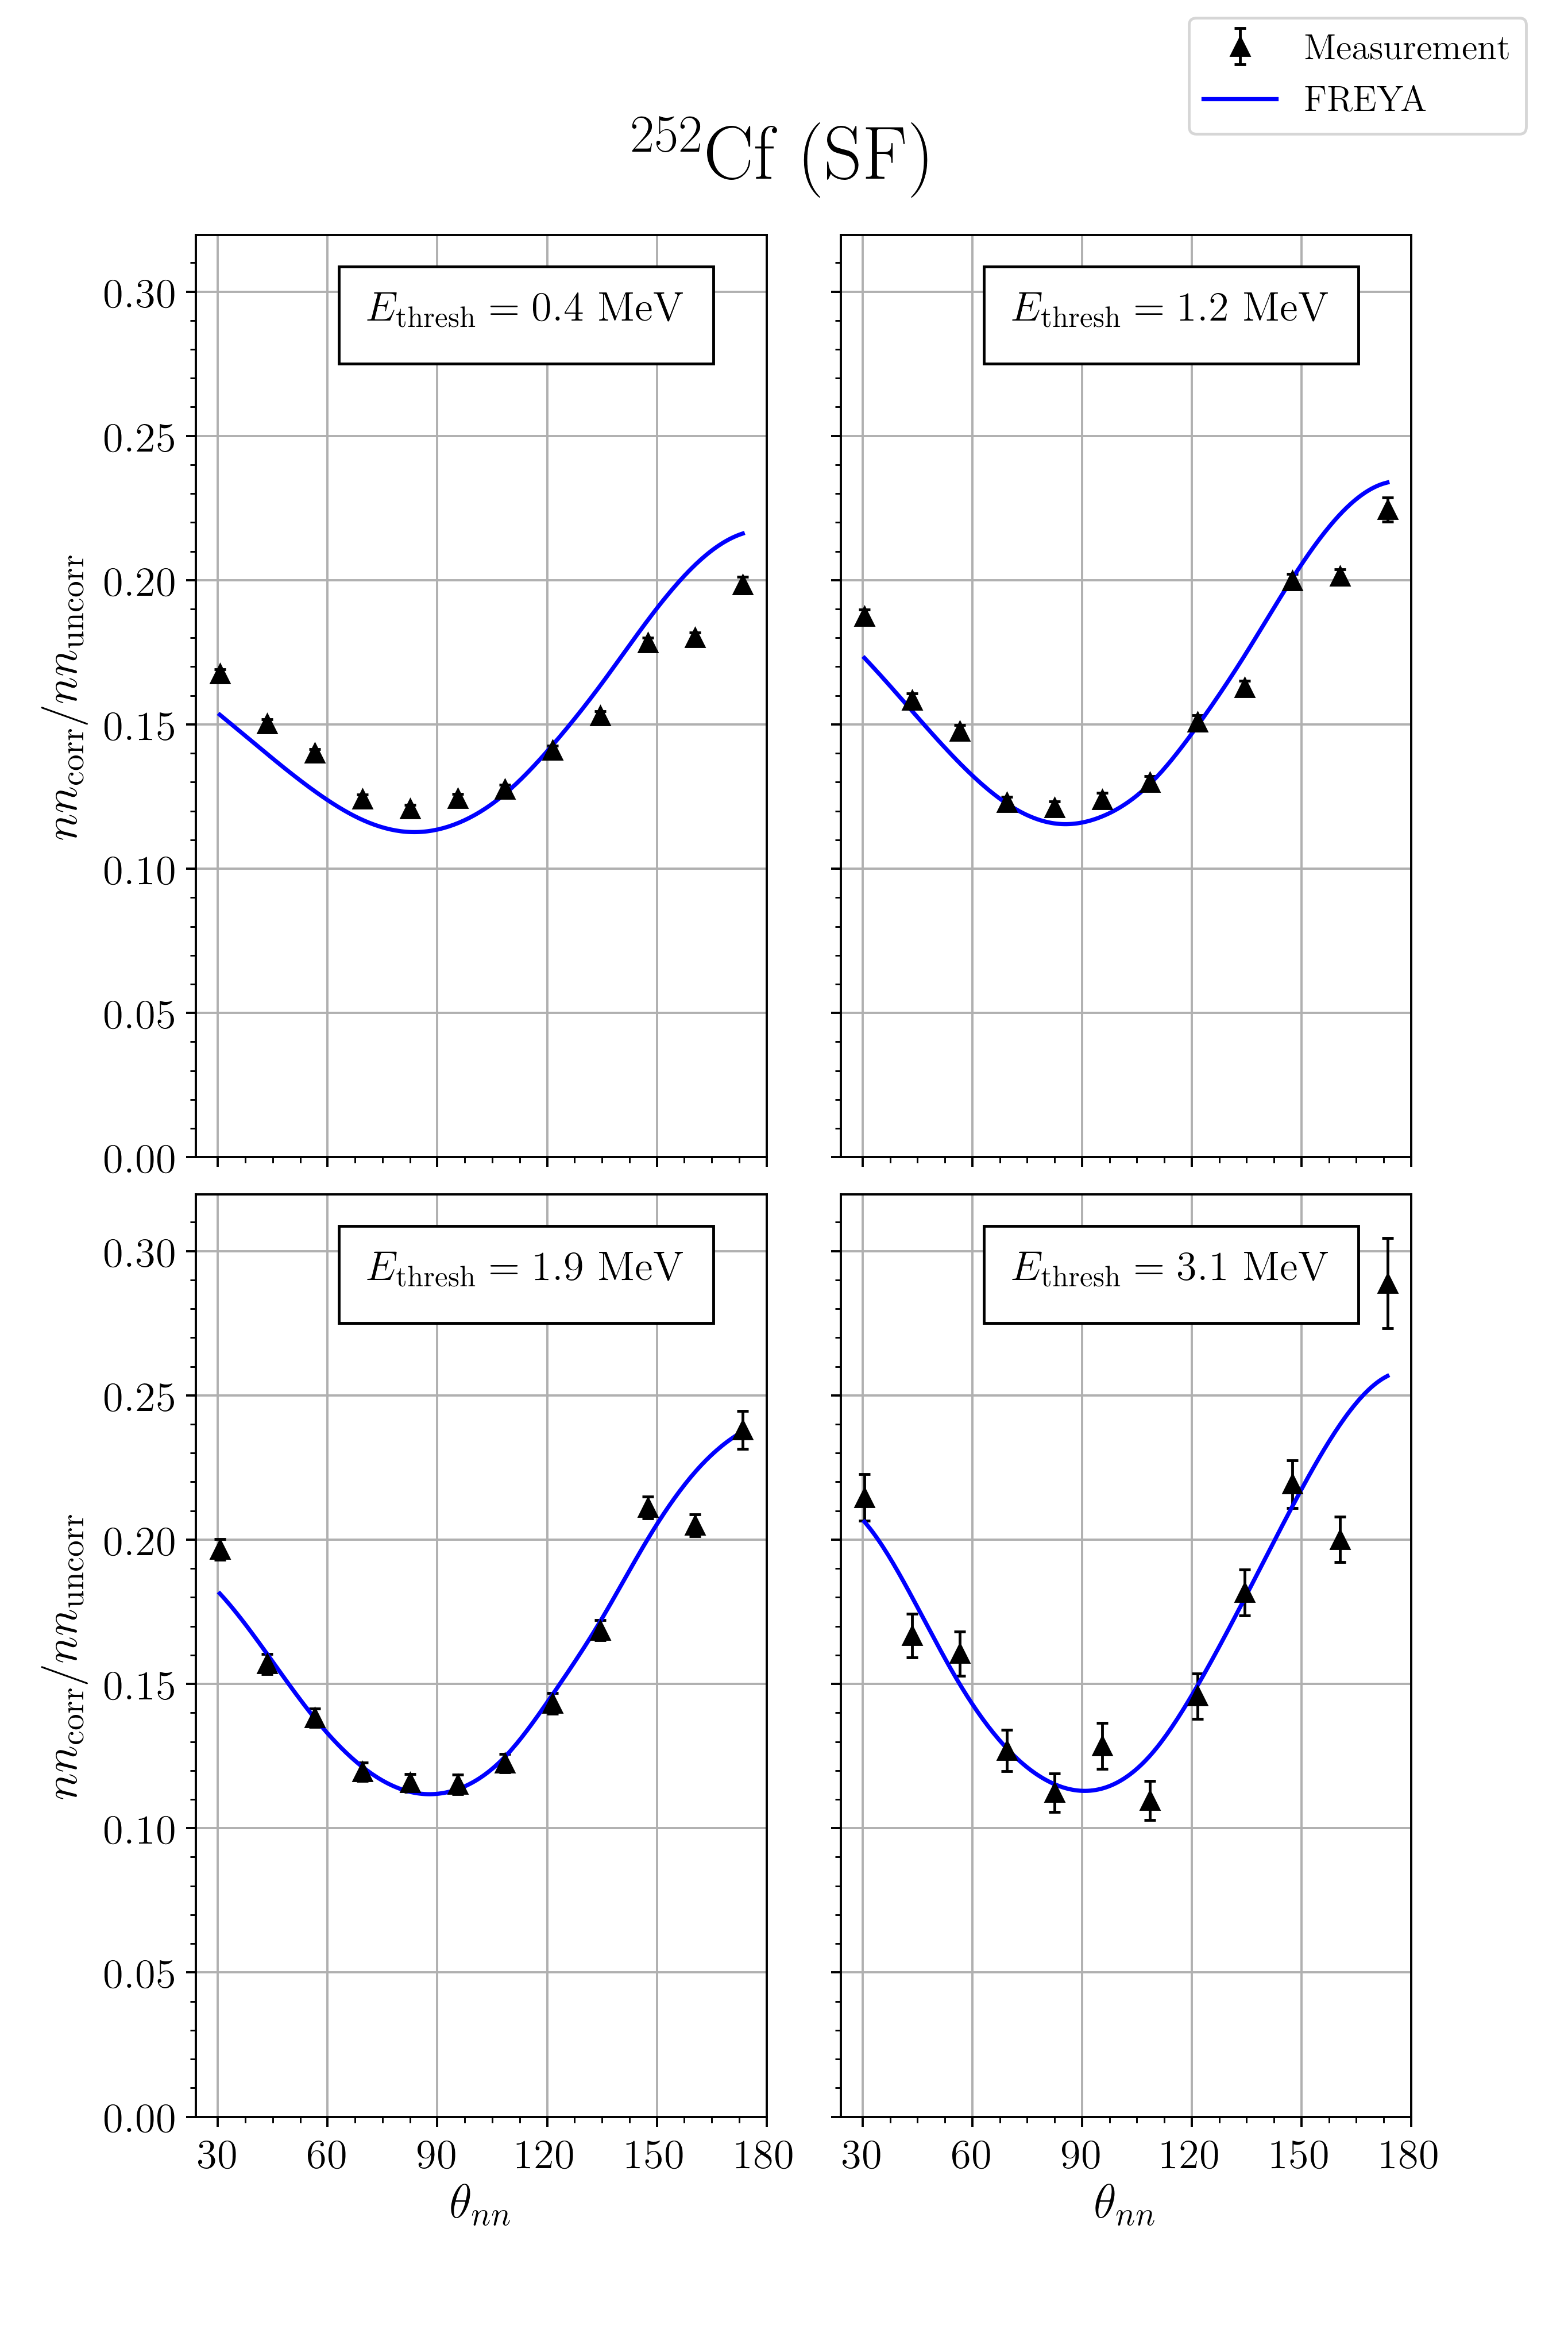
\includegraphics[width = 1.1\textwidth]{Content/Results/FinalCf252Resultw_freya0.png}
    \caption{}
    \label{fig:Cf(0)}
\end{figure}
\begin{figure}
\centering
    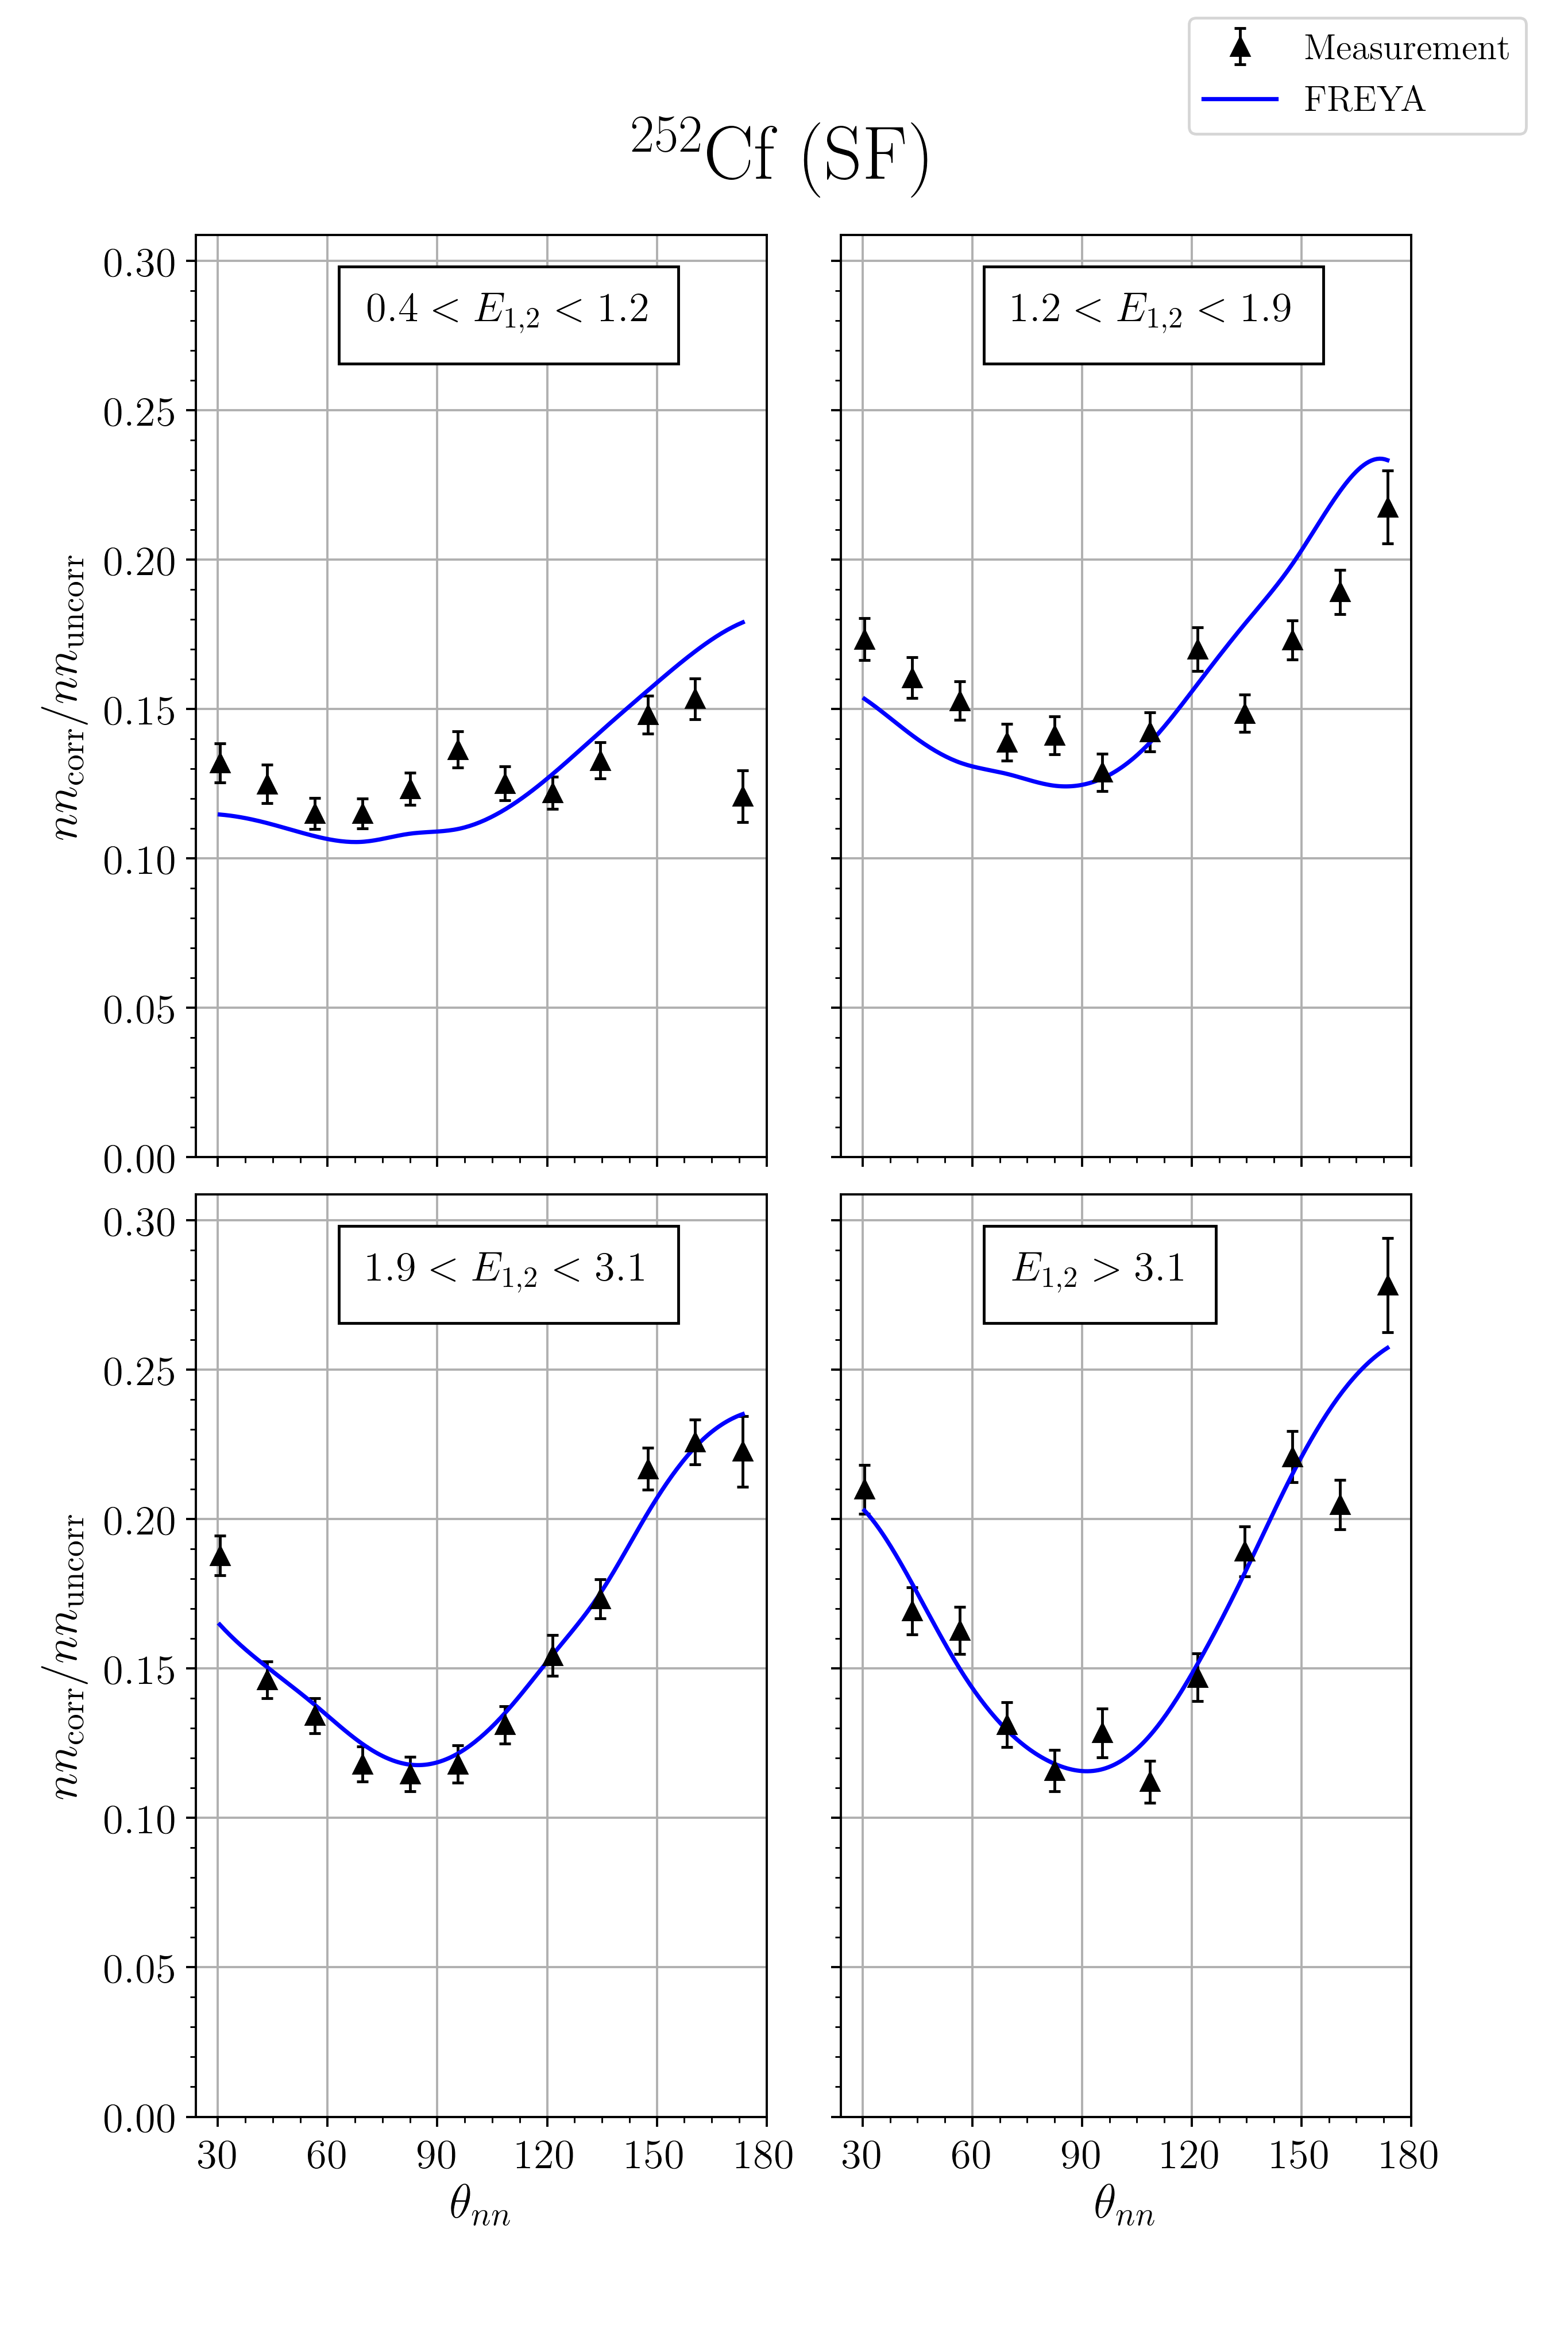
\includegraphics[width = 1.1\textwidth]{Content/Results/FinalCf252Resultw_freya2.png}
    \caption{}
    \label{fig:Cf(2)}
\end{figure}
\begin{figure}
\centering
    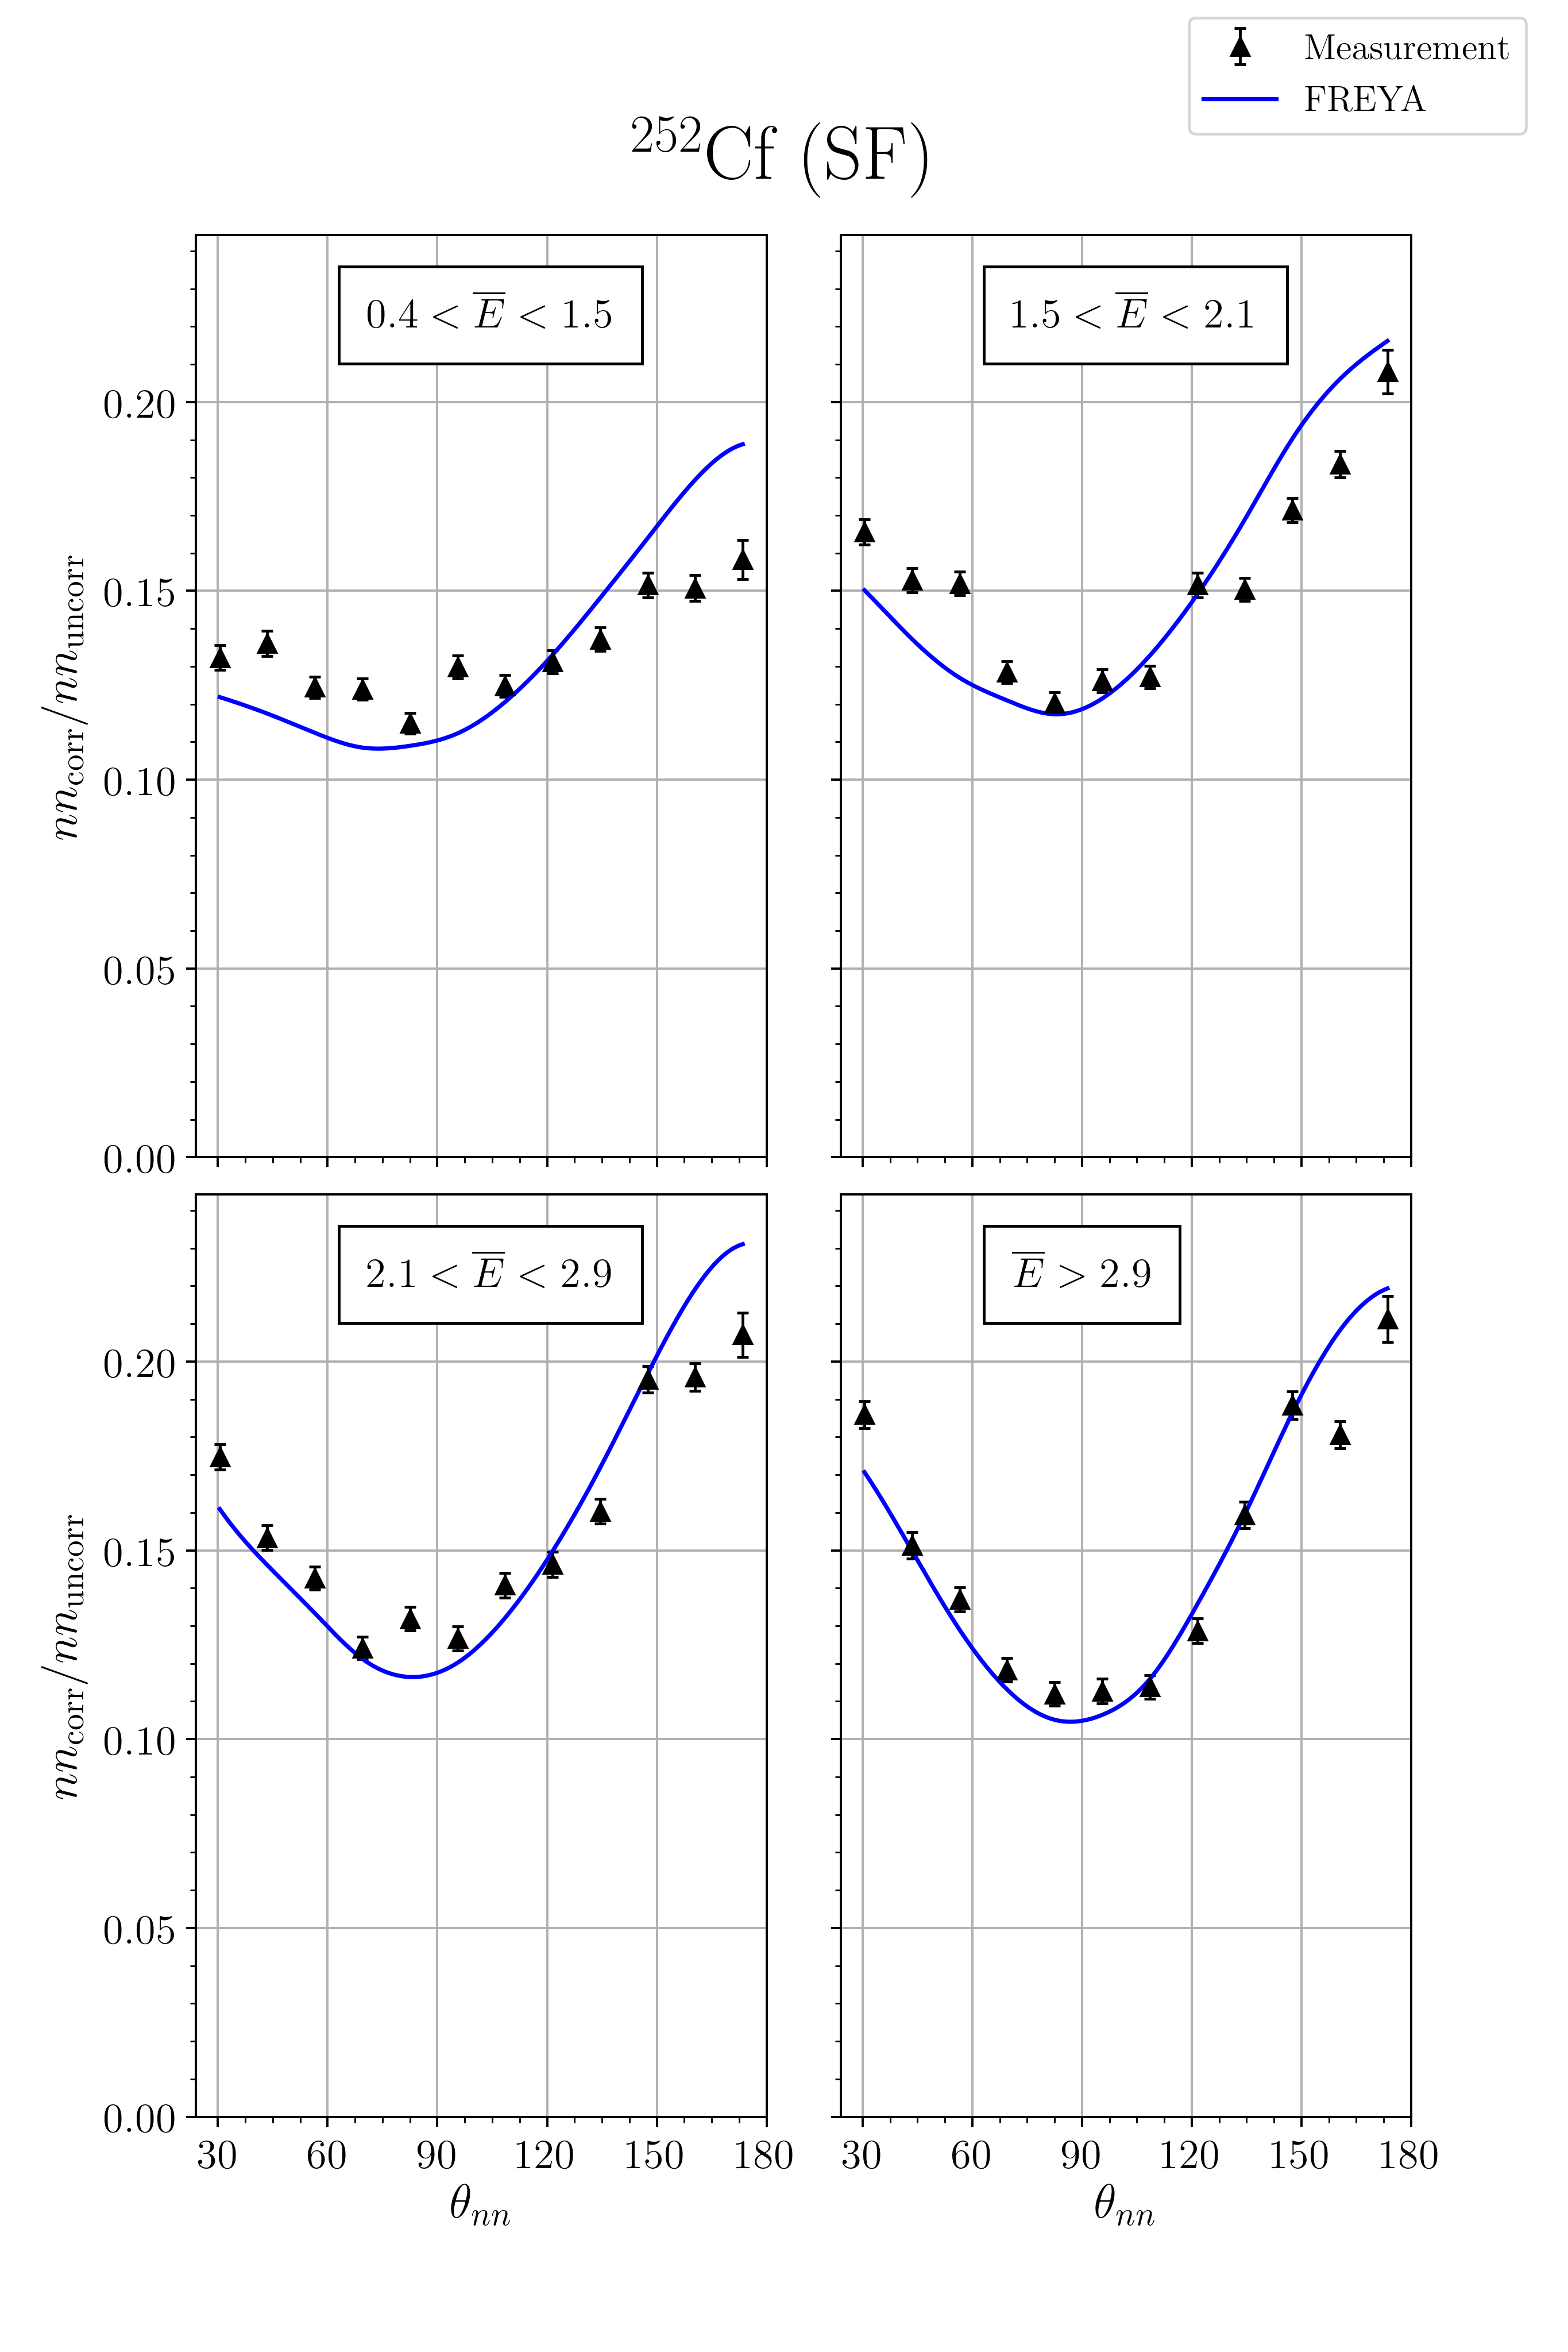
\includegraphics[width = 1.1\textwidth]{Content/Results/FinalCf252Resultw_freya1.png}
    \caption{}
    \label{fig:Cf(1)}
\end{figure}
\FloatBarrier


\section{Correlation of $\theta_{abs}$}
While these results are consistent with the effect of the kinematic focusing of the neutrons due to the recoil of the fission fragments, the data show a marked decrease in the two-neutron opening angle correlation in the region from about 165 to 180 degrees, which is well-pronounced in Fig.~\ref{fig:SPDPNormalization} and can also be seen in Figs~\ref{fig:FinalDUResult} and~\ref{fig:theta_abs_two_neutron}.
This feature is not evident in previous work on spontaneous and neutron induced fission.
As previously discussed, photofission differs from spontaneous and neutron induced fission in that the fission fragments for the photon induced reaction exhibit an asymmetry in their angle of emission, with the most likely orientation of the fission axis lying perpendicular to the direction of the incident photon.
With this in mind, the following series of angular cuts were made on the data.
Fig.~\ref{fig:theta_abs_LEGO} shows the distributions of absolute opening angles of the two-neutron events for three different cuts on the value of the two-neutron opening angle.
For two-neutron opening angles between 120 and 160 degrees, there is an increased preponderance of both neutrons being emitted around 90 degrees, consistent with the interpretation of kinematic focusing of neutrons coming from fission fragments which are themselves being emitted preferentially at 90 degrees.
However, in the opening angle region where the two-neutron correlation is reduced, from about 160 to 180 degrees, this feature is less prominent.

Furthermore, if one plots the opening angle distributions for the case in which at least one neutron is emitted perpendicular to the incident photon versus the case in which neither neutron is emitted perpendicular to the incident photon (Fig.~\ref{fig:theta_abs_two_neutron}), one sees that the two-neutron correlation is greatly reduced at 180 degrees in opening angle when at least one of the neutrons is emitted along the preferred fission axis.

These data are consistent with two possible explanations.
First, it is possible that there is a decrease in neutron emission along the fission axis.
Second, the neutrons may indeed be emitted isotropically in the rest frame of the fission fragment, but one fragment essentially shadows the neutrons emitted from the other fragment, either through absorption or scattering.
A definitive interpretation of this decreased two-neutron correlation for large opening angles in photo-fission requires further study.

\begin{figure}
    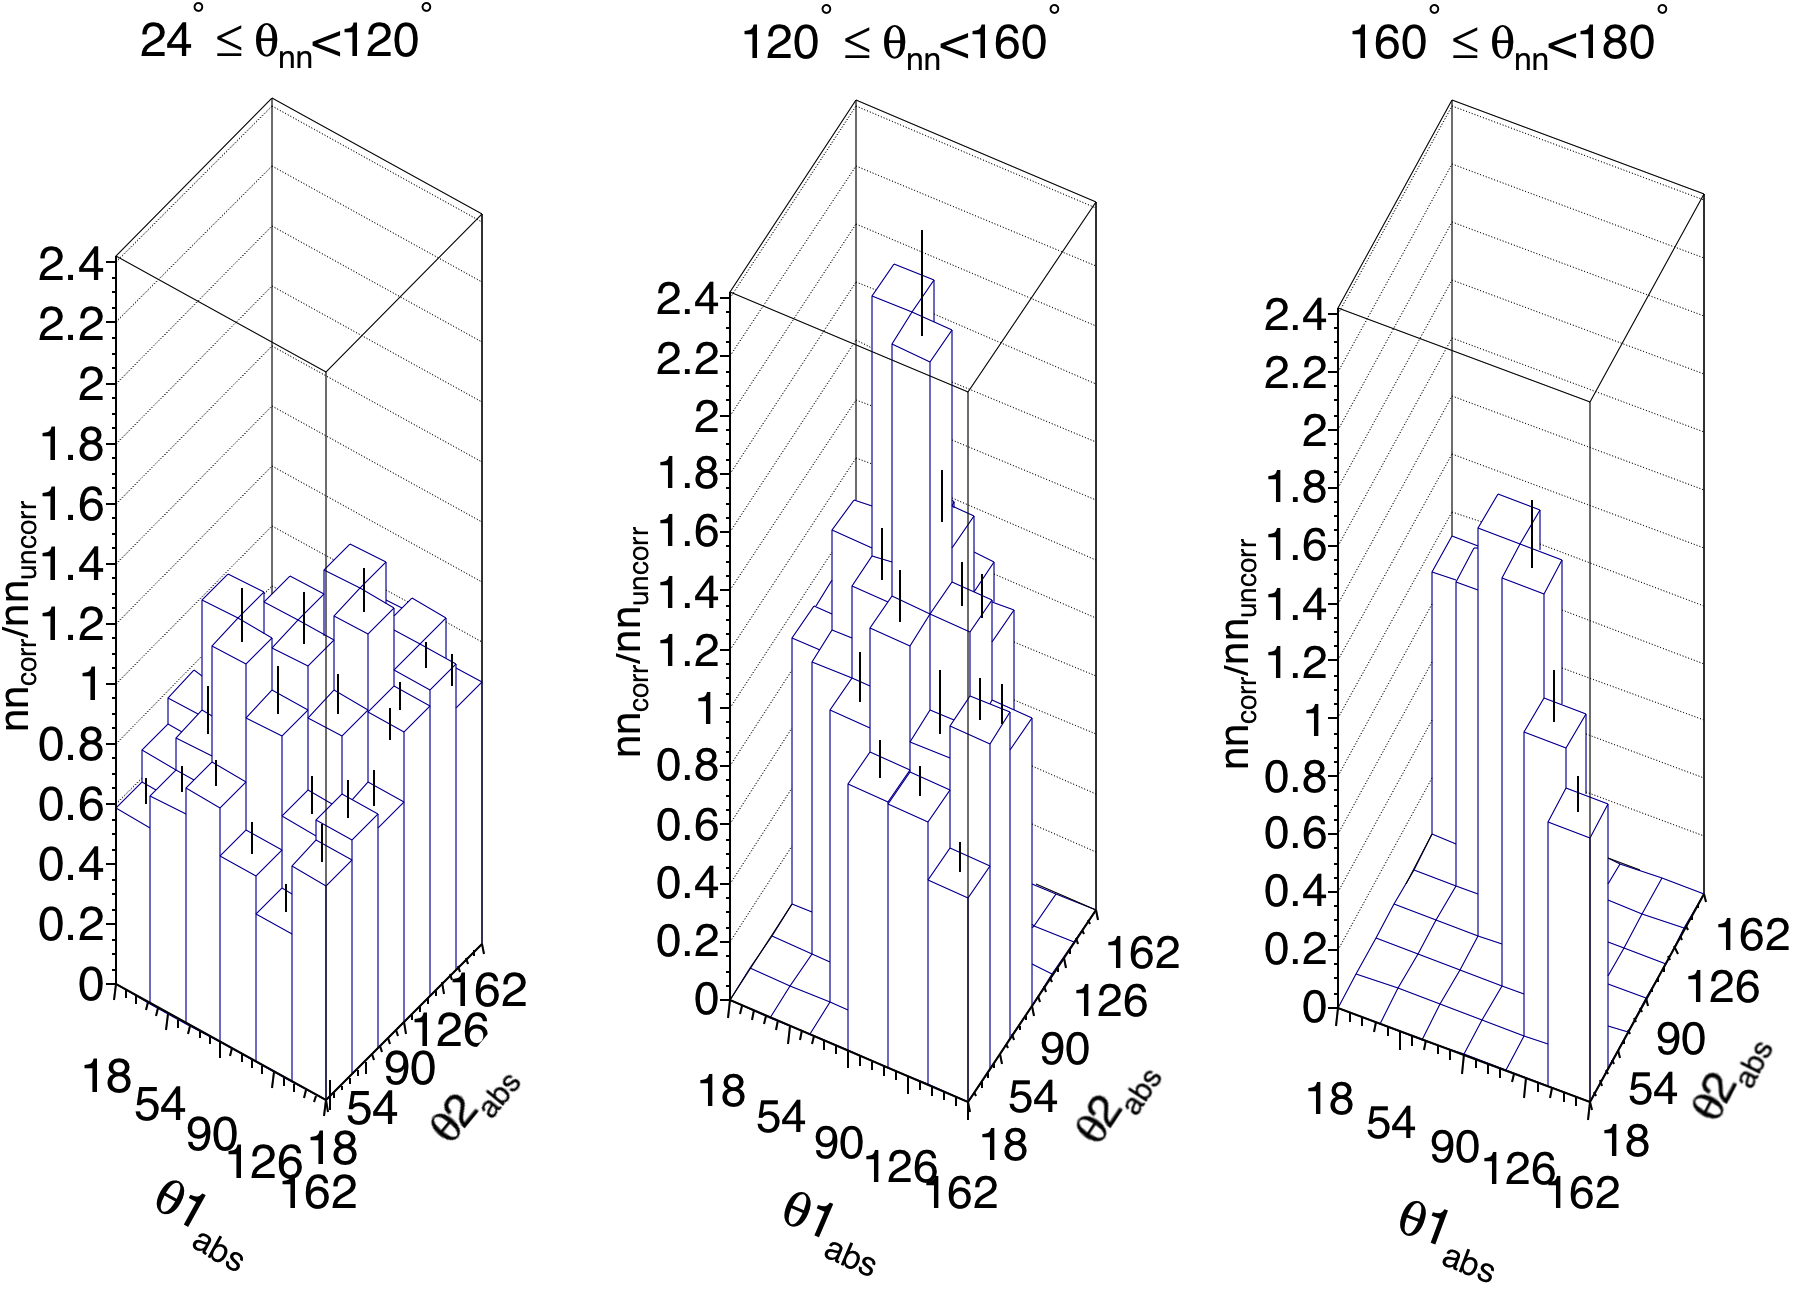
\includegraphics[width = 0.9\textwidth]{Content/Results/theta_abs_LEGO.png}
    \caption{Correlation is shown between the angles of each neutron with respect to the incident photon beam, denoted by $\theta 1_{abs}$ and $\theta 2_{abs}$.
    Empty bins exist because of incomplete $\theta_{abs}$ coverage.}
    \label{fig:theta_abs_LEGO}
\end{figure}
\begin{figure}
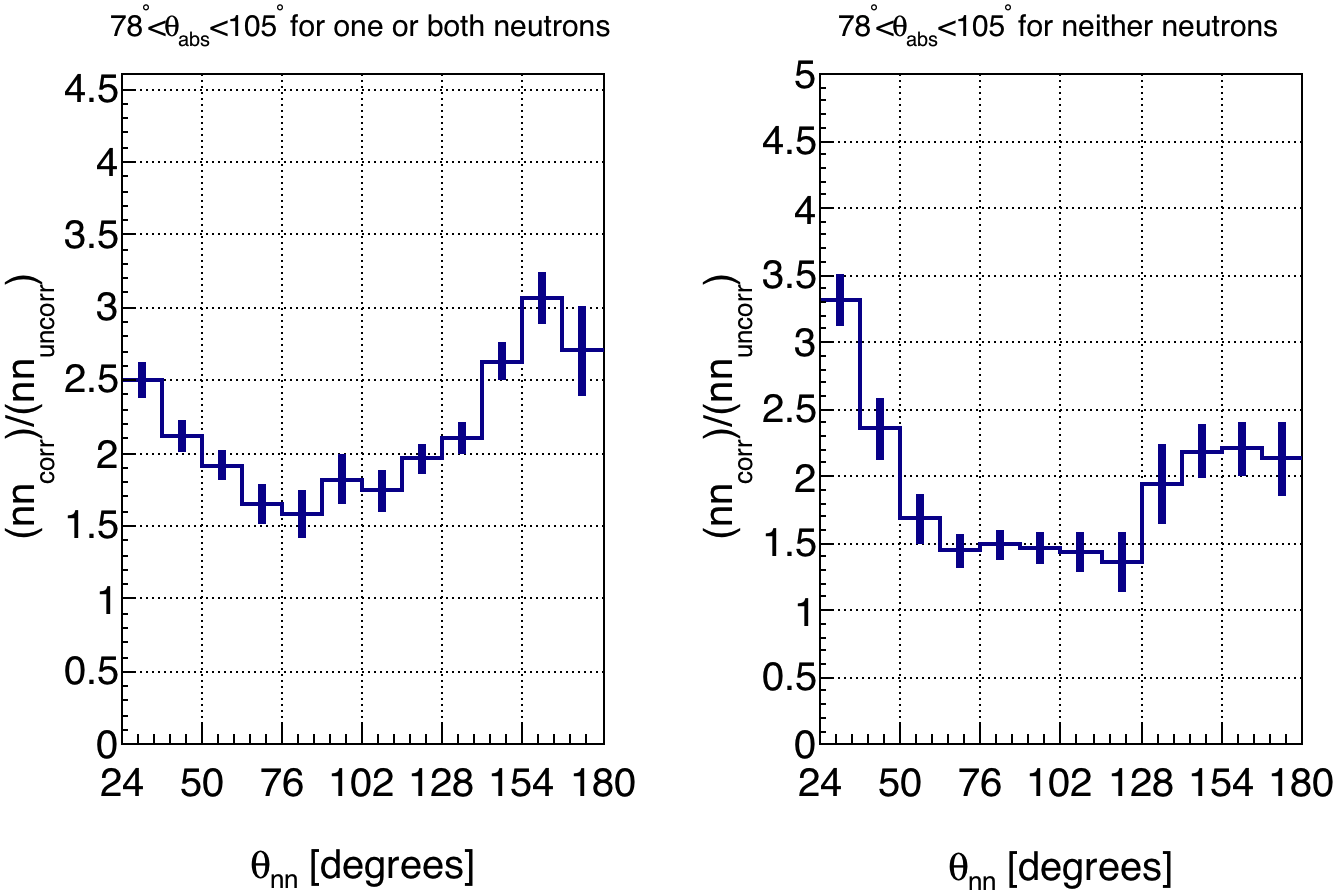
\includegraphics[width=0.9\textwidth]{Content/Results/theta_abs_two-neutron.png}
\caption{Requiring that at least one of the coincident neutrons be emitted nearly perpendicular to the photon beam (left) produces an opening angle distribution that is different from that produced when requiring that both neutrons are emitted nearly parallel to the photon beam (right).}
\label{fig:theta_abs_two_neutron}
\end{figure}

\FloatBarrier 
